\section{資訊檢索}
資訊檢索的目的是幫助使用者迅速地在資料庫中找尋所需要的文件。典型的資料檢索系統流程如圖~\ref{fig:chap2_retrieval}:首先,當使用想要找尋與某個主題(Topic)或概念(Concept)相關的文件時,使用者會先在腦中將所想的概念轉化成查詢詞,這裡的查詢詞長度不一,可以像一個句子、數個詞、單詞、或是字均可。根據系統設計的不同,查詢詞也可以是圖、照片、聲音、影片等皆可。
\begin{figure}
\centering
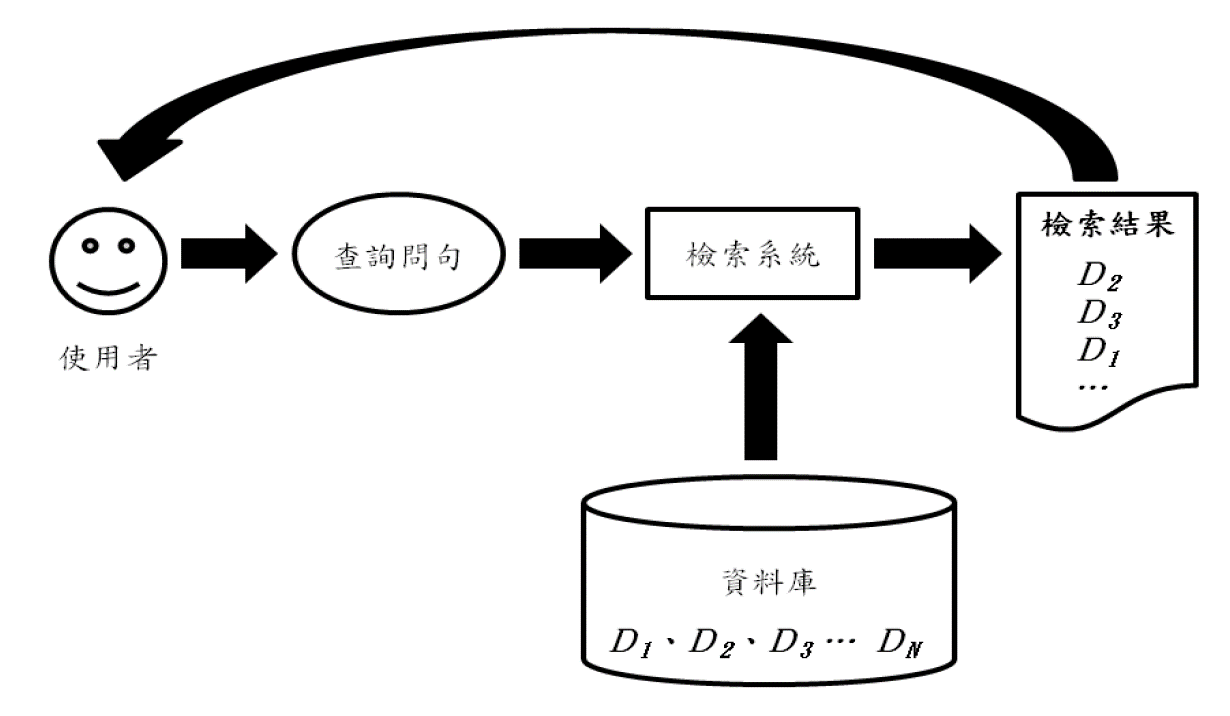
\includegraphics[scale=0.5]{images/chap2_retrieval.png}
\caption{資訊檢索的基本架構} \label{fig:chap2_retrieval}
\end{figure}

在得到查詢詞之後,系統會依照查詢詞$Q$與資料庫中的文件$D$計算相關分數$S(Q, D)$,一個系統的好壞通常決定於計算的相關分數是否準確。相關分數可以如下計算:

\[
S(Q, D) = P(r|Q, D)
\]

此處的$P(r|Q, D)$是代表當給定查詢詞$Q$和文件$D$時,兩者相關的機率有多少,這種排序方法稱為機率排序原則(Probability Ranking Principle, PRP)~\cite{amati2002probabilistic},而用來計算$P(r|Q, D)$的方法則有很多種,包括布林模型(Boolean Model)、向量空間模型(Vector Space Model)、機率模型(Probabilistic Model)~\cite{robertson1977probability}等。本論文使用的方法是基於語言模型的檢索(Language Model Based Retrieval)~\cite{chia2010statistical},先把查詢詞$Q$和文件$D$表示成兩個語言模型後,再計算兩個語言模型的KL散度 (Kullback–Leibler Divergence) 作為兩者的距離,具體作法見~\ref{subsec:retrievalsystem}節。
	
\subsection{口述語彙偵測與語意檢索}
語音檢索大致可分為兩大領域:口述語彙偵測 (Spoken Term Detection)~\cite{hazen2009query} 與語意檢索 (Semantic Retrieval)~\cite{lee2012improved} 。口述語彙偵測的目的是在所有語音文件集合中,找到包含語音查詢詞 (Spoken Query) $Q$ 的所有語音文件,語意檢索的目的是在所有語音文件集合中,找到語意上與語音查詢詞 $Q$ 相關 (Semantically Relevant)
的所有語音文件。舉例來說,如果使用者對系統說了:「美國總統」一詞,一個好的口述語彙偵測系統應該要能回傳所有包含「美國總統」一詞的語音文件,但一個好的語意檢索系統應該要能回傳所有包含「白宮」、「歐巴馬」等使用者覺得與查詢詞相關的詞的文件。由於語意檢索系統必須自動地猜測使用者可能想要找的詞彙,並主動尋找,因此存在有許多的挑戰,語意檢索將是此篇論文主要的研究主題。

\section{傳統語音資訊檢索}
語音資訊檢索系統大致上可以視為由兩個部分組成:語音辨識系統與資訊檢索系統。語音辨識系統需要有事先訓練好的聲學模型和語言模型,系統再從語音文件中抽出聲學特徵,系統再把聲學特徵辨識成為文字轉寫。有了文字轉寫之後檢索系統會計算查詢詞和各文件轉寫的相關性,再把此相關分數排序後回傳給使用者。

\subsection{語音辨識系統}
語音系統的目的是將語音訊號準確地轉寫成文字。典型的語音辨識系統流程包含了抽取語音特徵、訓練聲學模型和語言模型、產生辨識結果。

\subsubsection{抽取聲學特徵}
通常需要先抽取聲學特徵,再將聲學特徵辨識成文字,而目前最廣為使用的聲學特徵為梅爾倒頻譜係數 (Mel-Frequency Cepstrum Coefficient, MFCC)~\cite{huang2001spoken}。

\begin{figure}
\centering
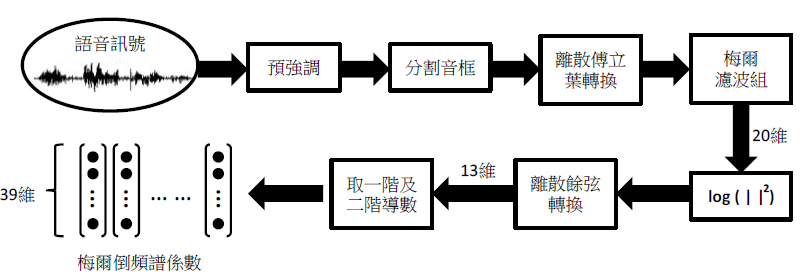
\includegraphics[scale=0.7]{images/chap2_mfcc.png}
\caption{梅爾倒頻譜係數抽取流程} \label{fig:chap2_mfcc}
\end{figure}

梅爾倒頻譜係數的抽取流程如圖~\ref{fig:chap2_mfcc}所示。第一步驟是預強調(Pre-emphasis)增加語音訊號裡高頻成分的比重。並且將語音訊號切成一連串長度固定且部分重疊的音框。再來,對每個音框內的訊號做離散傅立葉轉換,將每個音框內的訊號改為以頻率軸來表示。再把這些以頻率表示的訊號透過梅爾濾波組 (Mel-Filter Bank) 把每個音框壓縮成20維的向量。再把這些向量透過離散餘弦轉換 (Discrete Cosine Transform, DCT)
投射到彼此正交的軸上,此時可以忽略一些對訊號影響較小的維度,將訊號從20維降到12維,最後將音框中總體訊號能量相加後得到第13維。至此即可得到每個音框的13維向量,再對每個音框的13維向量取其一階與二階的時間軸導數 (Time Derivatives),即可形成39維的梅爾倒頻譜係數。

\subsubsection{訓練聲學模型}
\begin{figure}
\centering
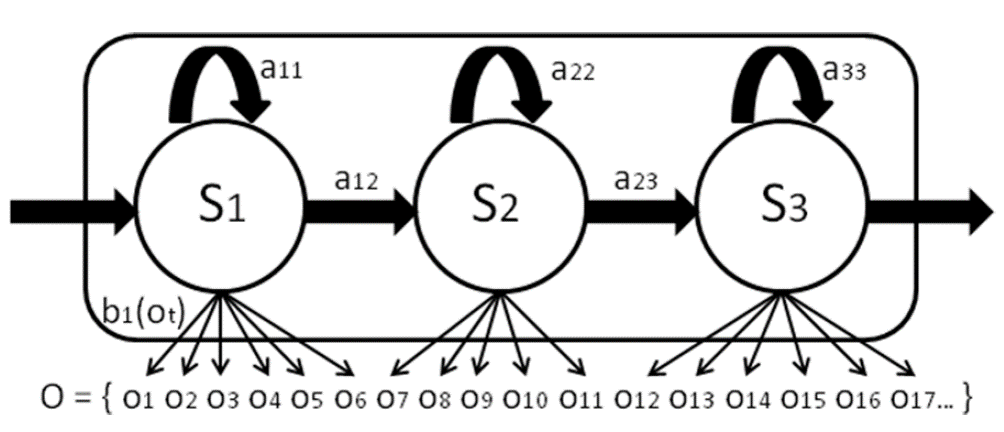
\includegraphics[scale=0.5]{images/chap2_hmm.png}
\caption{隱藏式馬可夫模型示意圖} \label{fig:chap2_hmm}
\end{figure}
訓練聲學模型最經典的方法即為隱藏式馬可夫模型 (Hidden Markov Models, HMM) ,其架構如圖~\ref{fig:chap2_hmm}  所示。隱藏式馬可夫模型是以一連串的狀態 (State) 模擬聲音隨時間轉換的特性。一個隱藏式馬可夫模型可以用來表示一個詞、字、音素、甚至是更小的聲學單位。而通常最常用的是三連音素是指每個狀態代表一個發音狀態。假設輸入的訊號為 $O = {o_t, t = 1, 2, 3, ...,
T}$,其中$O$代表一個語句,$o_t$為時間t的時候所對應到的聲學特徵,$T$則為語句的總長度。隱藏式馬可夫模型假設每個狀態之間有轉移機率 (Transition Probability),以$a_{ij}$表示從狀態$i$轉移到狀態$j$的機率:
    \begin{equation}
       a_{ij} = P(S_t = j | S_{t-1} = i)
    \end{equation}

$S_t$為$o_t$所屬的狀態,每一個狀態都是一個高斯混合模型 (Gaussian Mixture Model),用來表示在此狀態下聲學特徵的機率分布$b_j(o_t)$:
    \begin{equation}
    b_j(o_t) = P(o_t|S_t = j)
    \end{equation}
在此假設$o_t$只和當下的狀態$S_t$有關,而且狀態轉移只能停留在現在的狀態或是前往下一個狀態,無法後退或跳過一個狀態。

因此,一段聲音訊號$O$屬於某一段音素序列$w$的機率$P(O|w)$可表示為:
    \begin{equation}
    \begin{split}
       P(O|w) &= P(o_1o_2o_3...o_T | S_1S_2S_3...S_T) \\
              &= \Pi^T_{t=1}P(o_t|S_1S_2S_3...S_T) \\
              &= \Pi^T_{t=1}P(o_t|S_1S_2S_3...S_T) \\
              &= \Pi^T_{t=1}P(o_t|S_t, S_{t-1}) \\
              &= \Pi^T_{t=1}P(o_t|S_t)P(S_t|S_{t-1}) 
    \end{split}
    \end{equation}

    $w$是由一連串的狀態所構成,而$P(o_t|S_t)$可以用$b_j(o_t)$表示,$P(S_t|S_{t-1})$可以用$a_{ij}$來表示。這樣的聲學模型稱為隱藏馬可夫/高斯混合 (HMM/GMM) 模型。

\subsubsection{訓練語言模型}
語言模型是用來計算詞串$W$在某語言中出現的機率。假設$W = {w_1w_2...w_n}$,$w_i$代表在詞串$W$中出現的第$i$個詞彙,則$P(W)$可以表示成:
    \begin{equation}
        P(W) = P(w_1,w_2,w_3,...,w_n)
    \end{equation}
在此做個簡單的假設,詞彙$w_i$出現的機率會根據$w_i$前面的詞彙不同而有所差異。根據此假設將上式以條件機率展開則為:
    \begin{equation}
    P(W) = P(w_1, w_2, w_3,..., w_n) = \Pi^n_{k=1}P(w_k|w_1,w_2,...,w_{k-1}) 
    \end{equation}

    $w_1, w_2, ..., w_{k-1}$ 是$w_k$以前出現的詞彙,稱為歷史詞序列 (History Word Sequence),而$P(w_k| w_1, w_2, ..., w_{k-1})$則是$w_k$根據其歷史詞序列預測$w_k$出現的機率。

    如果歷史詞序列考慮的長度越長,所需的記憶體容量或硬體空間就越大,所以通常不會考慮很長的歷史詞序列。最常被使用的長度為詞雙連(Word Bigram)和詞三連(Word Trigram)的語言模型,分別對應到長度為2和3的歷史詞序列。因此詞雙連語言模型的機率可以近似為:
    \begin{equation}
    P(w_k|w_1, w_2, ..., w_{k-1}) \approx P(w_k|w_{k-1})
    \end{equation}

詞三連語言模型的機率可以近似為:
    \begin{equation}
    P(w_k|w_1, w_2, ..., w_{k-1}) \approx P(w_k|w_{k-2}, w_{k-1})
    \end{equation}

通常如果用來訓練語言模型的語料庫與要辨識的語句的領域越相近時,辨識結果會比較好,混淆度(Perplexity)也會越小。

\subsubsection{辨識結果}
把語音的訊號抽取出聲學特徵後,再經過聲學模型與語言模型計算出最佳的路徑後,即可得到此段語音的辨識結果,通常會將語音訊號辨識成兩種格式:詞圖(Lattice)~\cite{saraclar51lattice}和唯一最佳序列(One-Best
Transcription),詞圖像張網一樣,將每個時間所有可能的詞都呈現出來,而唯一最佳序列只呈現了詞圖上一條最可能的詞串當作辨識結果而已。通常在語音檢索時會使用詞圖來搜尋,因為語音辨識通常沒有辦法做到完全準確,可能會辨識成音很像的其他詞彙,比如「美國」可能會被辨識成「沒過」等等,如果使用唯一最佳序列的話,選中了正確的詞彙固然很好,但如果沒選中就會完全搜尋不出來了,而使用詞圖的話,這些可能的詞彙都會被表示在詞圖上,所以通常會使用詞圖來表示辨識的結果。

\begin{figure}
\centering
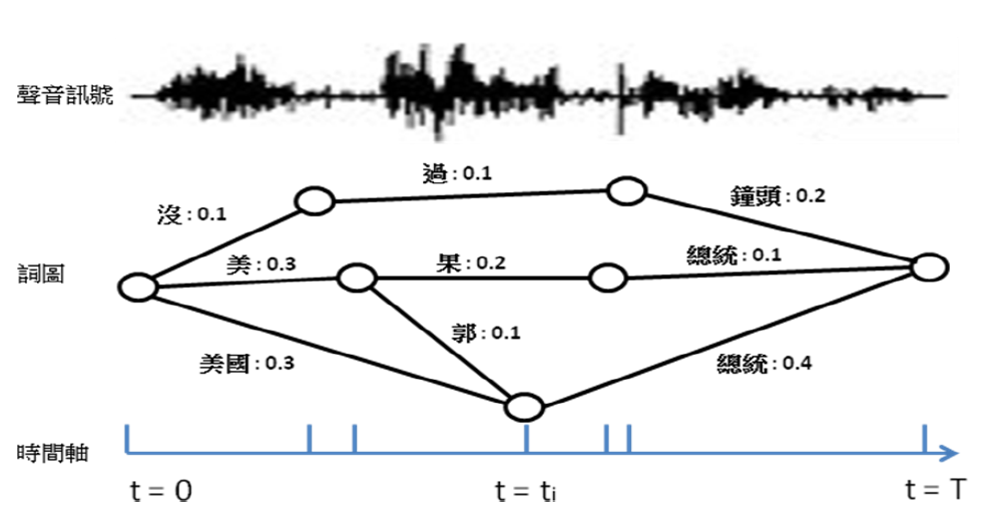
\includegraphics[scale=0.5]{images/chap2_lattice.png}
\caption{詞圖示意圖} \label{fig:chap2_lattice}
\end{figure}

如圖~\ref{fig:chap2_lattice}所示,詞圖主要由${N, A}$所構成,其中$N$是所有節點 (Node) 的集合,而$A$則是所有的詞弧 (Word Arc) 的集合。節點上存有各節點的時間資訊,而詞弧上除了有起始節點和終止節點外,還包含了在這個詞弧上的假定詞 (Word Hypothesis) 與此假定詞的信心分數 (Confidence Score) ,而此假定詞和信心分數都是由聲學模型和語言模型所計算出來的。

語音辨識系統的輸入是聲學特徵,並找出最有可能的詞彙串。因此相當於最大化以下的式子:
    \begin{equation}
    w^*_{seq} = argmax_{w_{seq} \in W_{seq}}P(w_{seq}|O)
    \end{equation}
O為輸入訊號之聲學特徵,$w_{seq}$為某個詞串,$W_{seq}$為所有$w_{seq}$之組合,$argmax$則是尋找一個$w_{seq}$使得$P(w_{seq}|O)$最大,此$w_{seq}$即為$w^*_{seq}$。但$P(w_{seq}|O)$無法直接被計算,所以根據貝氏定理 (Bayes' Theorem),可以表示如下:
    \begin{equation}
    P(w_{seq}|O) = \frac{P(O|w_{seq})P(w_{seq})}{P(O)}
    \end{equation}
由於$P(O)$是常數,可以不考慮,上式可簡化成:
    \begin{equation}
    P(w_{seq}|O) = P(O|w_{seq})P(w_{seq})
    \end{equation}

可以看得出來,$P(O|w_{seq})$可以由聲學模型求得,$P(w_{seq})$可以從語言模型中求得。求出來的$w^*_{seq}$即為唯一最佳序列。有時也會使用N最佳序列 (N-Best List) ,概念與唯一最佳序列很像,只是找出前N個讓$P(w_{seq}|O)$ 最大的$w_{seq}$。

\subsection{檢索系統}
\label{subsec:retrievalsystem}
檢索系統的目的主要是當使用者輸入查詢詞$Q$時,系統能夠計算出每個文件$X$與查詢詞間的相關分數$S(Q, X)$,進而將此相關分數排序後回傳給使用者。當系統接收到語音訊號時,系統會先對其抽取出聲學訊號,再經過聲學模型和語言模型辨識成唯一最佳序列或詞圖,一般來說,語音檢索系統使用詞圖的表現會比較好,所以以下主要就如何計算出查詢詞和詞圖的相關分數$S(Q, X)$加以介紹。

由於本章的檢索方式主要是基於語言模型的檢索 (Language model based retrieval)~\cite{zhai2008statistical, chia2010statistical},因此首先要把辨識所得的詞圖轉換為語言模型。對每個詞圖中的詞$t$,它在詞圖中的期望出現次數 (Expected Count) 可以如此計算:

\begin{equation}
E[t|x] = \sum_{\mu \in L(x)} N(t, \mu)P(\mu|x)
\end{equation}

$L(x)$是$x$的詞圖中所有的路徑,$\mu$是$L(x)$中的一條路徑,$N(t, \mu)$是$t$在$\mu$中出現的次數,$P(\mu|x)$是路徑$\mu$的事後機率(Posterior Probability)。

有了$E[t|x]$之後,就能把詞圖表示成單聯詞語言模型$\theta_x$:

\begin{equation}
P(t|\theta_x) = \frac{E[t|x]}{\sum_tE[t|x]}
\end{equation}

因為$\theta_x$裡沒有包含每個詞,為了讓$\theta_x$中每個詞都有一點機率,會再把$\theta_x$與一個背景語言模型 (Background Language Model) $\theta_b$做線性疊加,此過程稱為平滑化 (Smoothing)~\cite{zhai2001study},$\theta_b$可以如此估計:

\begin{equation}
P(t|\theta_b) = \frac{\sum_{x\in C}E[t|x]}{\sum_t\sum_{x\in C}E[t|x]}
\end{equation}

$C$ 是所有文件$x$的集合。

同樣地,查詢詞$Q$也可以被表示成語言模型$\theta_Q$:

\begin{equation}
P(t|\theta_Q) = \frac{N(t, Q)}{|Q|}   
\end{equation}

$N(t, Q)$是詞$t$出現在$Q$中的次數,而$|Q|$是$Q$中詞的總數。

有了$\theta_x, \theta_b, \theta_Q$之後,就可以計算$\theta_x$與$\theta_Q$之間的相關分數$S(x, Q)$了,由於$\theta_x, \theta_b, \theta_Q$都是機率分布 (Probability Distribution) ,所以在這裡選擇了KL散度 (Kullback–Leibler divergence) 用來計算兩個語言模型之間的距離,KL散度的計算方式如下:

\begin{equation}
KL(\theta_x | \theta_Q) = \Pi_{w\in V}P(w|\theta_x)^{P(w|Q)}
\end{equation}

於是定義文件$x$和查詢詞$Q$之間的相關分數$S(x, Q)$如下:

\begin{equation}
S(x, Q) = -[(1-w_1)KL(\theta_q^w|\bar{\theta}^w_x) + w_1KL(\theta_q^s|\bar{\theta}_x^s)]
\end{equation}

$\bar{\theta}_x$是將$\theta_x$與$\theta_b$疊加後的語言模型,上標$w$代表的是用以詞為基礎的詞圖產生的語言模型,上標$s$代表的是用以次詞單位 (Subword Unit) 為基礎的詞圖產生的語言模型,上式是分別對詞為基礎的語言模型和次詞為基礎的語言模型做檢索,再將兩者得到的相關分數用$w_1$做線性疊加,最後再將此分數排序後回傳給使用者。

\subsection{資訊檢索評估機制}
為了讓研究人員能夠比較彼此系統之成效,制定資訊檢索評估機制的標準是很重要的一環,本節將介紹此篇論文使用的評估機制。

\subsubsection{準確率(Precision)與召回率(Recall)}

準確率越高代表所找出的檢索結果越可靠,而召回率越高的話代表系統找回越多相關的檢索目標,通常會為系統設定一個閥值(Threshold),文件的分數若高於閥值,則視為相關,反之若文件的分數低於閥值,則視為不相關。準確率和召回率的定義如下:

\[
\text{準確率}=\frac{\text{檢索到的相關檢索對象數}}{\text{檢索到的檢索對象數}}
\]

\[
\text{召回率}=\frac{\text{檢索到的相關檢索對象數}}{\text{所有的相關檢索對象數}}
\]

通常這兩個值彼此之間的關係為負相關。調高閥值的話準確率會上升,但召回率則會下降;反之若調低閥值,準確率會因此下降,召回率則會很高。可以考慮一個極端例子:當閥值非常低時,幾乎所有的文件都是相關文件,此時的召回率相當於1,但準確率就會很低了。因此單看準確率或召回率是無法準確地評估系統的優劣的,必須要兩者一起評估。

\begin{figure}
\centering
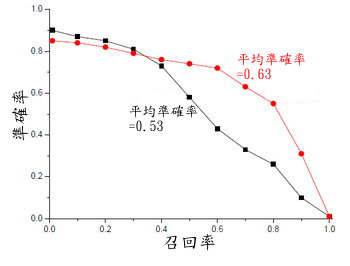
\includegraphics[scale=1.0]{images/chap2_precision_recall.png}
\caption{準確率、召回率和平均準確率之關係} \label{fig:precision_recall}
\end{figure}

\subsubsection{P@N}

通常使用者最重視的是檢索系統傳回的前幾名結果,所以就發展出了$P@N$這個評估機制。$P@N$就是只看前N個檢索結果的正確率。例如:前五個檢索結果中有一個是相關的,那$P@5$就是20\%。

$P@N$的定義如下:
\[
P@N=\frac{\text{前N個文件裡的相關文件數}}{N}
\]

\subsubsection{平均準確率~\cite{garofolo2000trec}}

因為準確率和$P@N$都需要事先決定,當查詢詞和條件不同時,很難準確地評估兩個系統的效能。因此有人提出了平均準確率(Mean Average Precision, MAP)的概念,如圖~\ref{fig:precision_recall},平均準確率就是準確率和召回率曲線下面積的平均值。平均準確率的定義如下:
\begin{equation}
MAP = \frac{1}{|Q|} \sum_Q \frac{\sum_{d \in D^R}precision(d)}{|D^R|}
\end{equation}
其中Q代表查詢詞的集合,$|Q|$為查詢詞的總數,$D^R$為和查詢詞Q相關的文件d的集合,$|D^R|$代表和查詢詞Q相關的文件數量。precision(d)代表系統檢索出文件d時的準確率。

\section{相關回饋}
相關回饋 (Relevance Feedback) 是資訊檢索的一項重要的技術~\cite{ruthven2003survey},通常可以顯著地提升系統的成果。相關回饋基本的架構如圖 ~\ref{fig:chap2_prf},使用者輸入查詢詞之後,系統會先根據查詢詞與所有文件的相關分數 $S(Q, d)$ 排序出第一次檢索結果 (First-pass Result)。然後把第一次檢索結果中部分文件標注為與查詢詞相關的正例 (Positive Example) ,部分文件標注為與查詢詞非相關的反例 (Negative Example)
,系統會再根據標注的結果重新計算查詢詞與文件的關係,把調整後的結果呈現給使用者看。
\begin{figure}
\centering
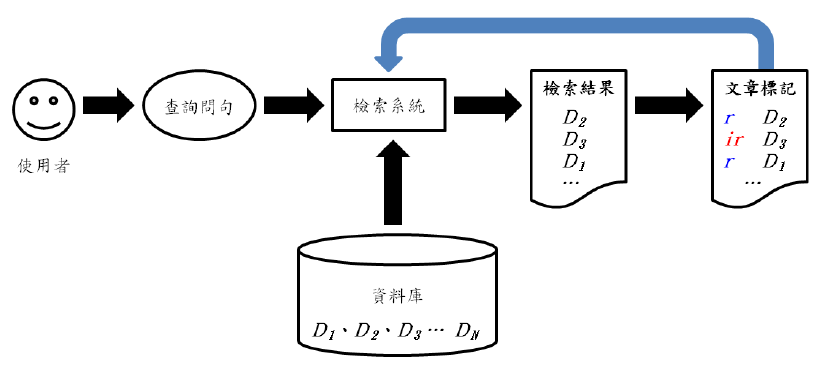
\includegraphics[scale=0.7]{images/chap2_prf.png}
\caption{相關回饋的基本架構} \label{fig:chap2_prf}
\end{figure}


把部分文件標注成正例與反例的方法可以大致分為以下幾種:

\subsection{外顯回饋}
外顯回饋 (Explicit Feedback) 的做法通常是由使用者告訴系統文件是否為正例或反例,進而增進檢索的成果。外顯回饋可分為使用者回饋 (User Feedback) 和積極回饋 (Active Feedback)
,使用者回饋是由使用者依據第一次檢索結果按照文件相關性進行標注~\cite{salton1975vector, zhai2001model, robertson1976relevance};積極回饋則是由系統主動詢問使用者某文件為正例或反例(通常是詢問系統無法決定的文件),此方法可以盡量減少使用者的標注量以改進系統的成果~\cite{tong2001support, goh2004multimodal, he2004mean}。

\subsection{隱含回饋}
隱含回饋 (Implicit Feedback) 是不由使用者直接提供正反例的資訊,而且透過觀察使用者的行為 (Behavior) 而分析文件的相關性,因此使用者並不知道自己正在回饋給系統。最常用的方法是點擊數據 (Click-through Data),比如檢索系統的前幾名如果是$d_1, d_2, d_3, ...$,而使用者沒有檢視$d_1$,而是直接檢視$d_2$,如此一來系統就可以假設$d_1$是不相關的文件,而$d_2$是相關的文件。除此之外,還可以利用查詢記錄 (Query Log)、網頁捲動
(Scrolling)和滑鼠軌跡 (Mouse Movements) 等~\cite{kelly2003implicit}。

\subsection{虛擬回饋}
虛擬回饋 (Pseudo Feedback) 不需要使用者的參與,在系統產生第一次檢索結果後,系統會直接假設其中某些部分為正例,某些部分為反例(通常是直接假設相關分數最高的$N$篇為正例,相關分數最低的$N$篇為反例)。系統會再根據這些假設進行進一步的檢索,在這個過程中,系統雖然沒有得到額外的資訊,但系統的成效通常能有一定的提升~\cite{kurland2005better, xu1996query, yu2003improving, sakai2005flexible, cao2008selecting, lee2008cluster, lv2009comparative, lv2010positional},而虛擬回饋也是此篇論文的主要研究主題之一。

\section{本章總結}
本章介紹了資訊檢索的背景,包含了基礎的資訊檢索架構、口述語彙偵測與語意檢索的差別,以及相關回饋的基本概念,並介紹了語音檢索系統的兩個主要的部分:辨識系統與檢索系統,最後介紹了動態時間扭曲做為口述語彙偵測的方法。
